\documentclass{article}
\usepackage{fullpage}
\usepackage{graphicx}
\graphicspath{{../images-videos/}}  
\usepackage{titlesec}
\usepackage{amsmath}
\usepackage{amssymb}
\usepackage{array}
\usepackage{float}
\usepackage{xcolor}
\usepackage{hyperref}  % Optional for clickable ToC
\usepackage{ulem} 
\usepackage{caption} % per usare \caption fuori dall'ambiente figure
\renewcommand{\baselinestretch}{2}
\author{Paradiso Emiliano,  \quad 1940454 \\Piccione Brian, \quad 1889051 \\Pisapia Vittorio,  \quad 1918590 }
\title{\Huge Medical Robotics project \\ \centering \Large \textbf{Shared control of a teleoperated echographic probe}}

\hypersetup{
    colorlinks=true,            % Collega con colori invece che riquadri
    urlcolor=blue,              % Colore dei collegamenti ipertestuali
    linkcolor=black 
}

\titleformat{\chapter}[block]
  {\normalfont\LARGE\bfseries} 
  {}                           
  {0pt}                      
  {\LARGE}        
   
\begin{document}

\date{}
\maketitle
\vspace{-1cm}

\begin{figure}[h]
    \centering
    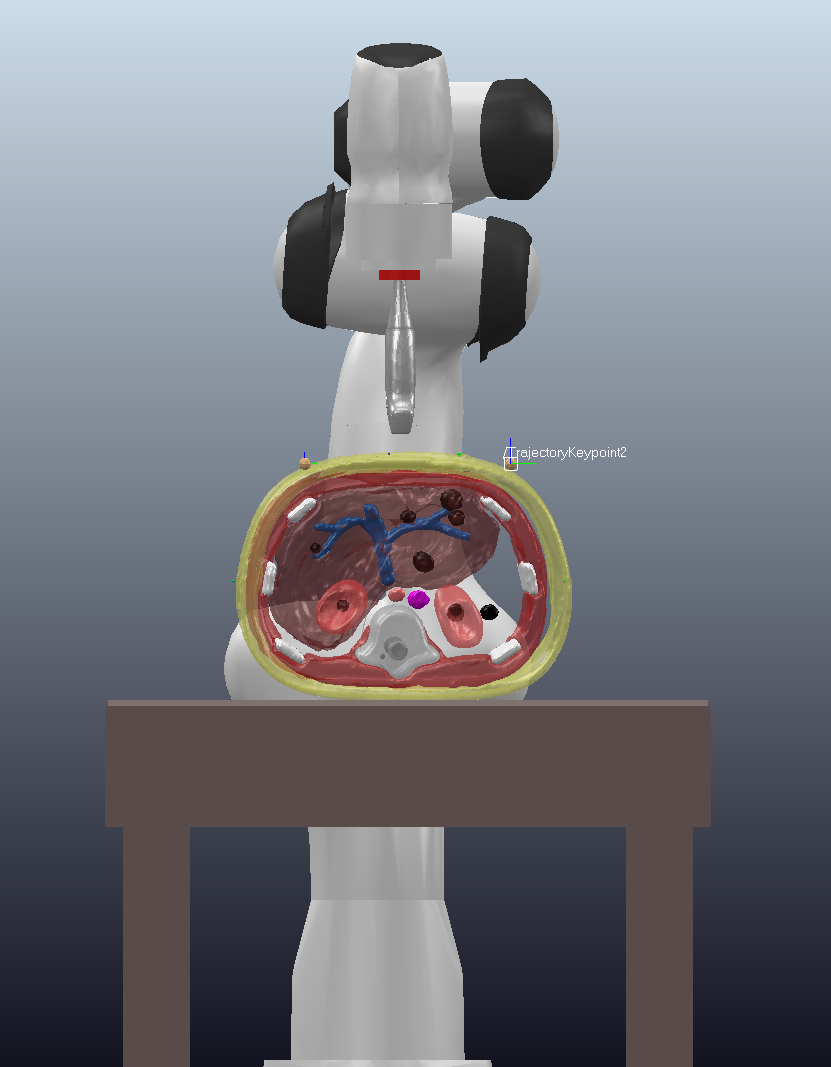
\includegraphics[width=0.25\textwidth]{Approach.png}  
    %\caption{}
    %\label{Approach}
\end{figure}

\begin{abstract}
%% SCRIVI L'ABSTRACT
\hspace*{-0.5cm}This work focuses on developing a shared control system for a teleoperated echographic probe integrated with the Franka Emika Panda Robot. To achieve this, we will derive an impedance control law that meets the compliance requirements for the specified tasks. We will then implement a shared control architecture to enhance the collaboration between the manipulator and the human operator. Additionally, we will design several trajectories and approaches for the scanning task, ensuring it can be performed safely and autonomously. This study aims to demonstrate the advantages of shared control in critical scenarios, where effective collaboration between human and robot is essential for precise task execution and the prevention of hazardous situations.
\\GitHub link: \uline{\href{https://github.com/VittorioPisapia/Medical-Robotics/tree/main}{https://github.com/VittorioPisapia/Medical-Robotics/tree/main}}
\end{abstract}

\newpage
\tableofcontents
\newpage

\section{Problem introduction}
Echography, or ultrasound imaging, is a widely used medical technique with applications in cardiology, abdominal imaging, and fetal monitoring during pregnancy. It is highly valued because it is non-invasive and generally safe for people of all ages.
However, the quality and accuracy of echography are often operator-dependent, meaning they rely heavily on the skill and experience of the person performing the scan. Different operators may produce varying results. Additionally, operators may not always follow the exact same path or apply consistent pressure, leading to variability in image quality, particularly in follow-up examinations, where consistency is crucial for monitoring changes in a patient's condition over time.
These limitations are a primary reason why robot-assisted echography is gaining popularity. Robotic systems are designed to operate with precise control, ensuring consistent pressure application and accurate movement paths during the scan. 
However, despite its advantages over conventional echography, robot-assisted echography is still under development and tends to be more costly than its traditional counterpart. One of the key challenges in developing a robot-assisted echography system is controlling the probe during the echographic task. Although forces must be exchanged to perform the scan, the contact forces between the robot and the patient must be limited to ensure the patient’s safety. This can be done by implementing an impedance control law.
A crucial improvement in this area is the implementation of shared control systems, which facilitate the remote operation of echographic probes by expert clinicians. Shared control refers to a collaborative approach where both the human operator and the robotic system work together to perform a task. This paradigm enhances the efficiency, safety, and precision of teleoperated procedures by leveraging the strengths of both human intuition and robotic accuracy.
The clinician can intervene in real time to adjust the probe's position or to focus on specific areas of interest, while the robot ensures that movements are executed smoothly and safely. This balance of control not only improves the quality of the ultrasound examination but also alleviates the physical strain on the operator.
This report will explore the underlying principles and advantages of this technology. We will examine the impact of shared control on the workflow of tele-echographic procedures and its implications for future developments in robotic-assisted medical applications. Through this exploration, we aim to highlight the critical role that shared control plays in advancing the field of telemedicine and improving patient outcomes.


\section{State of the Art}
In this chapter, we will examine various works and systems related to tele-echography. Our focus will be on providing detailed descriptions of three specific systems. 

\subsection{The TER system}
Among the various tele-ultrasound systems, TER is a tele-robotic system consisting of a master workstation (with or without force feedback control) and a slave robot operated remotely by a clinician to perform ultrasound-based diagnoses. The master system has been developed and tested with two approaches: one using a position sensor with visual feedback, and another incorporating a haptic device for force feedback. A unique feature of TER is its slave system, which is actuated by artificial muscles, giving it natural compliance.

\begin{figure}[h]
    \centering
    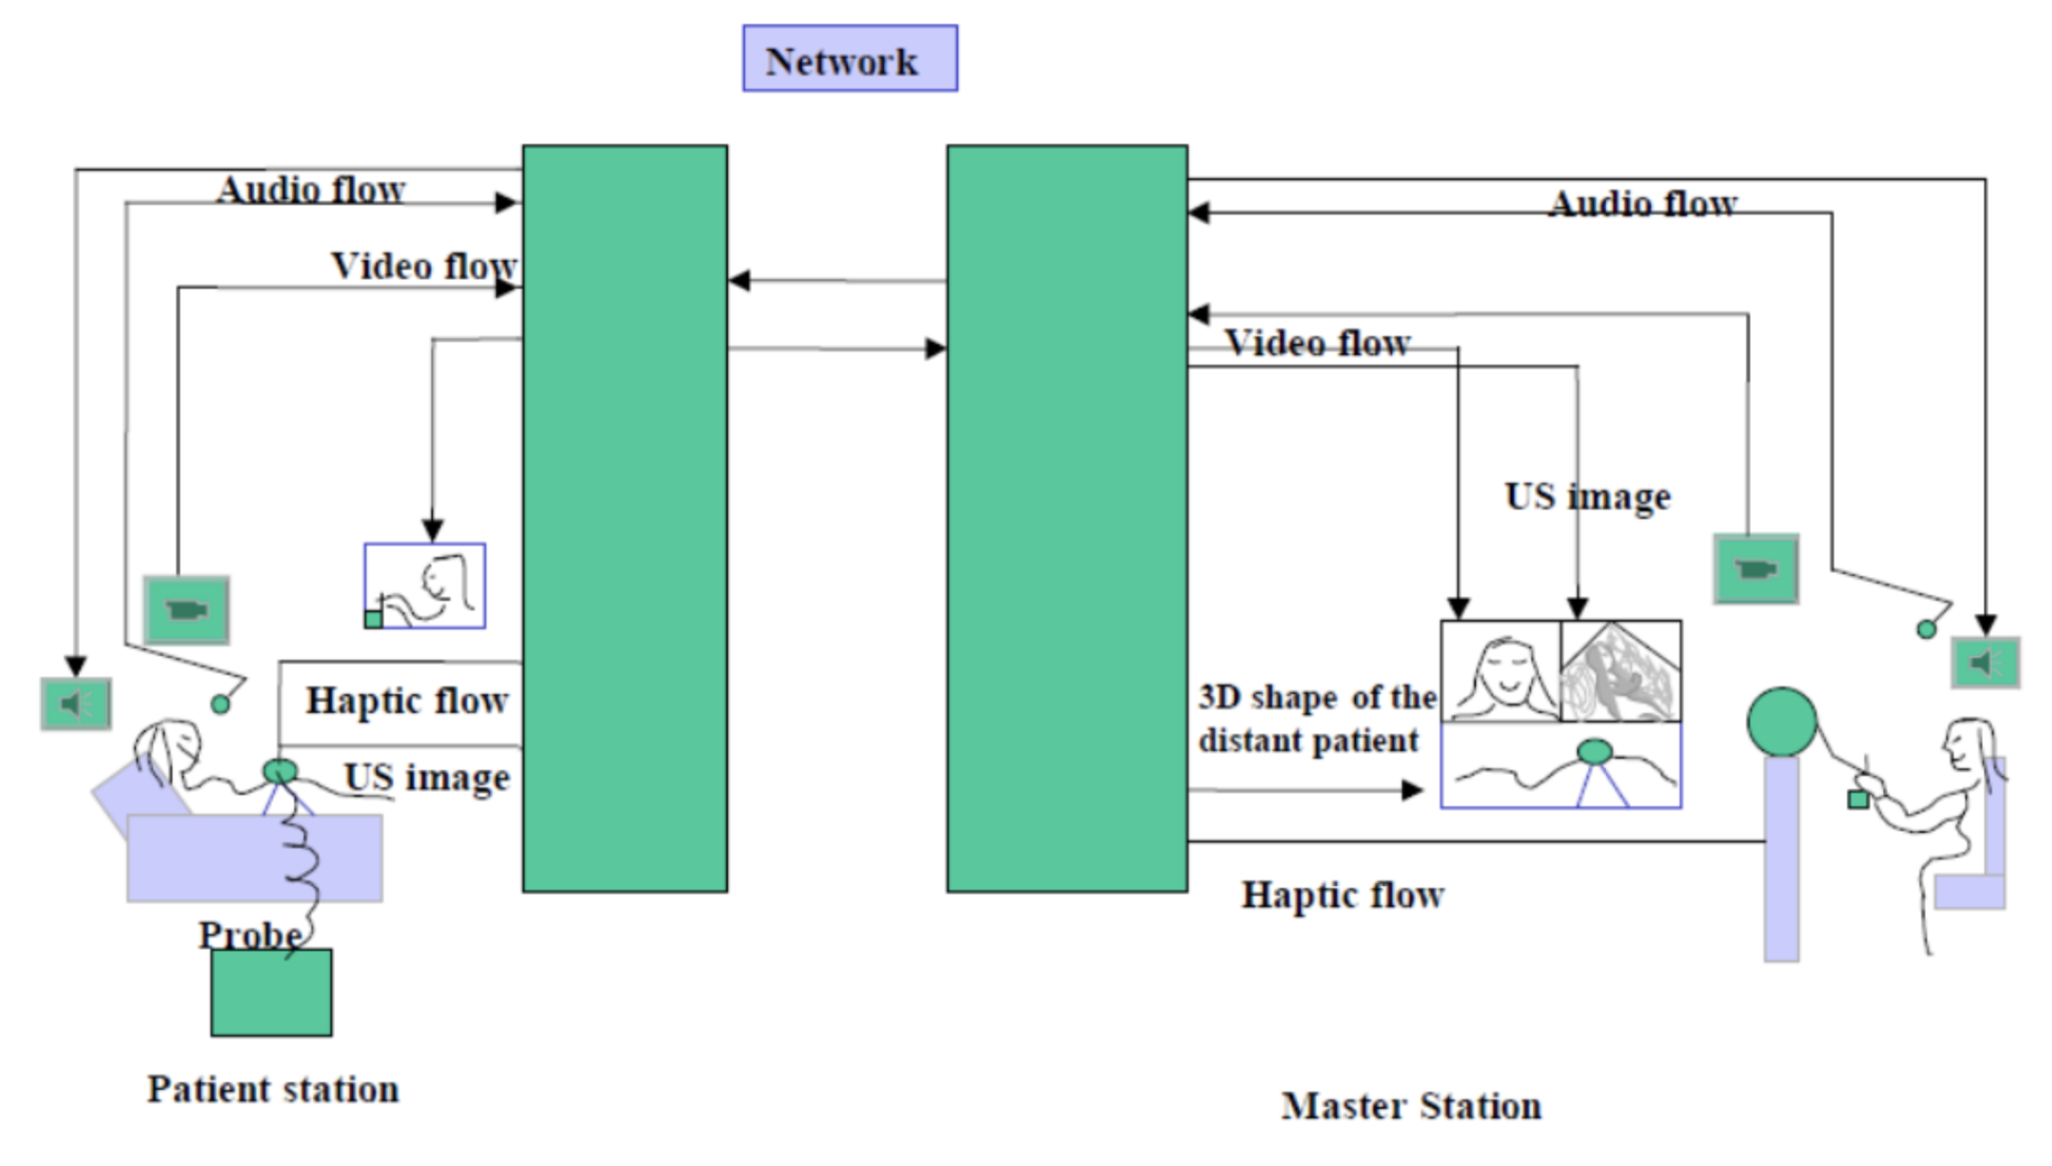
\includegraphics[width=0.7\textwidth]{TER.png}  
    \caption{TER architecture}
    \label{fig:ter}
\end{figure}


\subsection{The MELODY system}
The system operates under a long-distance paradigm, allowing for remote teleoperated ultrasound examinations, such as from a central hospital to a local facility or an isolated location. This approach offers several advantages, including increased access to specialized healthcare for remote communities and more cost-effective service delivery.
\\The system comprises three primary components: the expert system (master station), the patient system (slave station), and the communication link that facilitates data exchange between these two stations.

\begin{figure}[h]
    \centering
    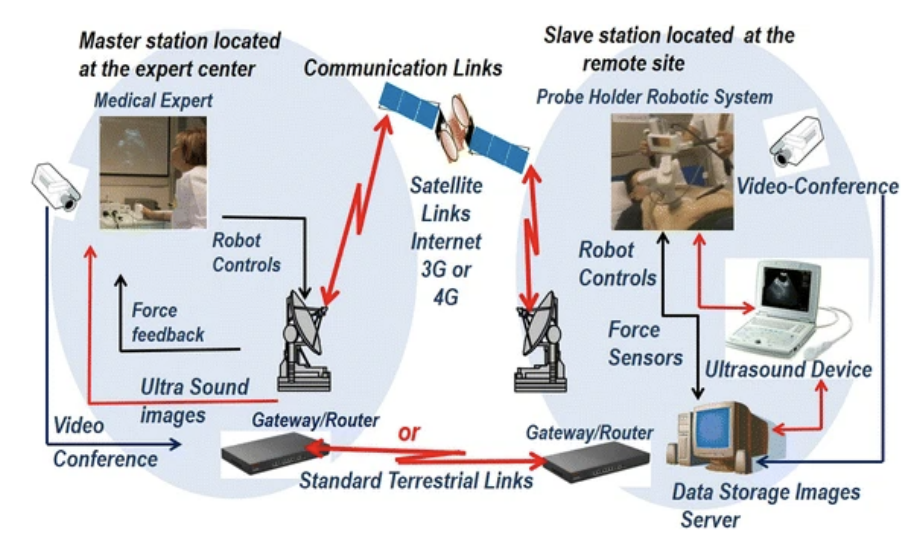
\includegraphics[width=0.7\textwidth]{MELODY.png}  
    \caption{The MELODY system}
    \label{fig:melody}
\end{figure}

\subsection{The OTELO system}
OTELO is a remotely operated system designed to perform reliable ultrasound imaging at a distant, isolated location without the need for a specialist clinician on-site. It is a mobile tele-echography solution utilizing an ultra-light robot, comprising three key components:

%\renewcommand{\labelitemi}{-}

\begin{itemize}
\item The expert site, where a doctor controls the positioning of the remote robot using a dedicated haptic probe. This probe mimics the feel and function of a traditional ultrasound probe, familiar to medical professionals, enhancing ergonomic comfort. The doctor also receives feedback on the contact force between the probe and the patient's skin, thanks to a force sensor located in the probe holder system.
\item The communication link, which can be either satellite or terrestrial, facilitates data transmission between the two locations.
The patient station, consisting of a lightweight 6-degree-of-freedom robotic system and its control unit. \item This robot manipulates the ultrasound probe in response to commands from the medical expert. It is maintained by a nurse or a non-specialist assistant, who positions and holds the robot on the patient’s skin under the guidance of the doctor via videoconference. The robot replicates the movements of the virtual probe on the real ultrasound probe.
\end{itemize}

\begin{figure}[h]
    \centering
    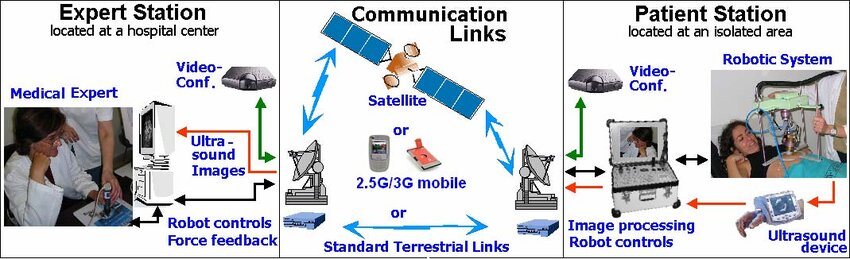
\includegraphics[width=0.7\textwidth]{OTELO.png}  
    \caption{The OTELO system}
    \label{fig:otelo}
\end{figure}


\begin{figure}[h]
    \centering
    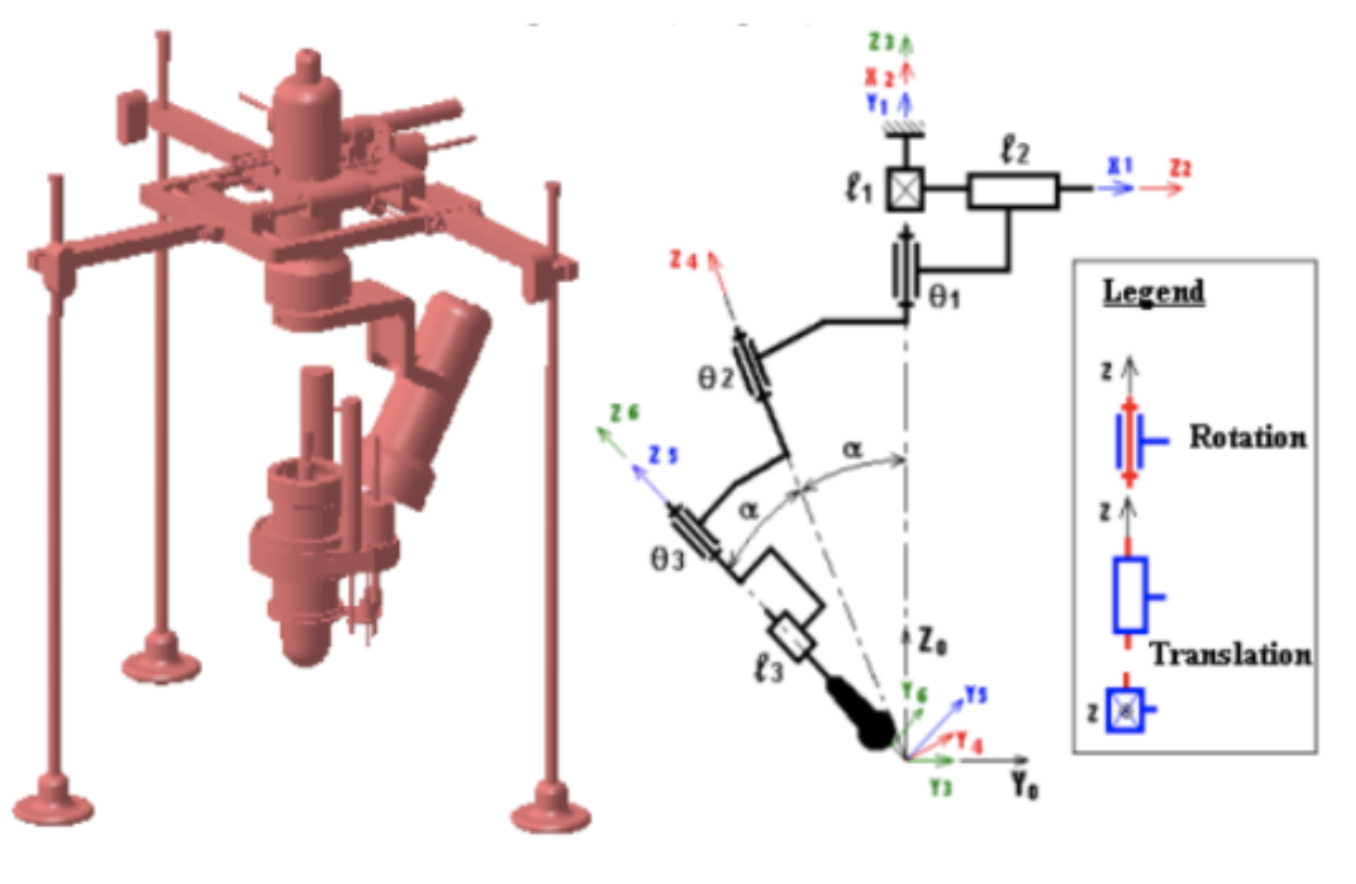
\includegraphics[width=0.5\textwidth]{OTELO_structure.png}  
    \caption{Mechanical structure of OTELO 1}
    \label{fig:otelo struc}
\end{figure}

\subsection{A previous project on related work}
Our colleagues implemented an impedance control system for a manipulator designed to perform a tele-echography task $\cite{Colleagues}$. The simulated manipulator is equipped with an ultrasound probe that interacts with an abdominal phantom. Starting from an initial position above the phantom, the probe approaches the abdomen perpendicularly and then slides across its surface while maintaining low contact forces.

\paragraph{Limitations:}
\begin{itemize}
\item The previous work did not fully achieve teleoperated motion under shared control, as it was limited to implementing pre-defined trajectories.
\item The robot's redundancy was not utilized to keep its structure at a safe distance from the patient, which is important for ensuring optimal safety during task execution.
\item No force/torque sensors were used in CoppeliaSim to measure the contact forces during the simulation.
\end{itemize}
\par

\section{Development}
This section outlines the approach used to achieve the task, with a particular emphasis on the formal formulation of the control law, the implementation of shared control, and a brief explanation of the implemented trajectories.

%%TASK DEFINITION
\subsection{Task definition}
To ensure a safe and accurate scan, the task vector is defined as a 6-component vector. The first three components represent the x, y, and z cartesian coordinates of the end-effector, which are determined using the robot's direct kinematics. The fourth element corresponds to the z-coordinate (expressed in the world frame) of the fourth joint: by adjusting its height, it is possible to avoid collisions with the patient and prevent potentially hazardous configurations during the scan. This component is computed using partial direct kinematics. The final two elements describe the orientation, defined using ZYZ Euler angles around the Z (phi) and Y (theta) axes. 
The angles have been defined by equating the rotation matrix derived from the robot's direct kinematics from the robot’s base to the end-effector, with the composition of three elementary rotations around the moving ZYZ axes:
$$
R(\phi,\theta,\psi)=\begin{pmatrix}
c_{\phi}c_{\theta}c_{\psi}-s_{\phi}s_{\psi} & -c_{\phi}c_{\theta}s_{\psi}-s_{\phi}c_{\psi} & c_{\phi}s_{\theta}\\
s_{\phi}c_{\theta}c_{\psi}+c_{\phi}s_{\psi} & -s_{\phi}c_{\theta}s_{\psi}+c_{\phi}c_{\psi} & s_{\phi}s_{\theta}\\
-s_{\theta}c_{\psi} & s_{\theta}s_{\psi} & c_{\theta}
\end{pmatrix}
$$
Then the task vector is:
\newline
\noindent
\begin{minipage}{0.4\textwidth}
\hspace{1cm}
   $
    r=\begin{pmatrix}
    x\\
    y\\
    z\\
    \theta\\
    z^{\text{4th}}\\
    \phi
    \end{pmatrix}
    $
\end{minipage}%
\begin{minipage}{0.5\textwidth}
    \centering
    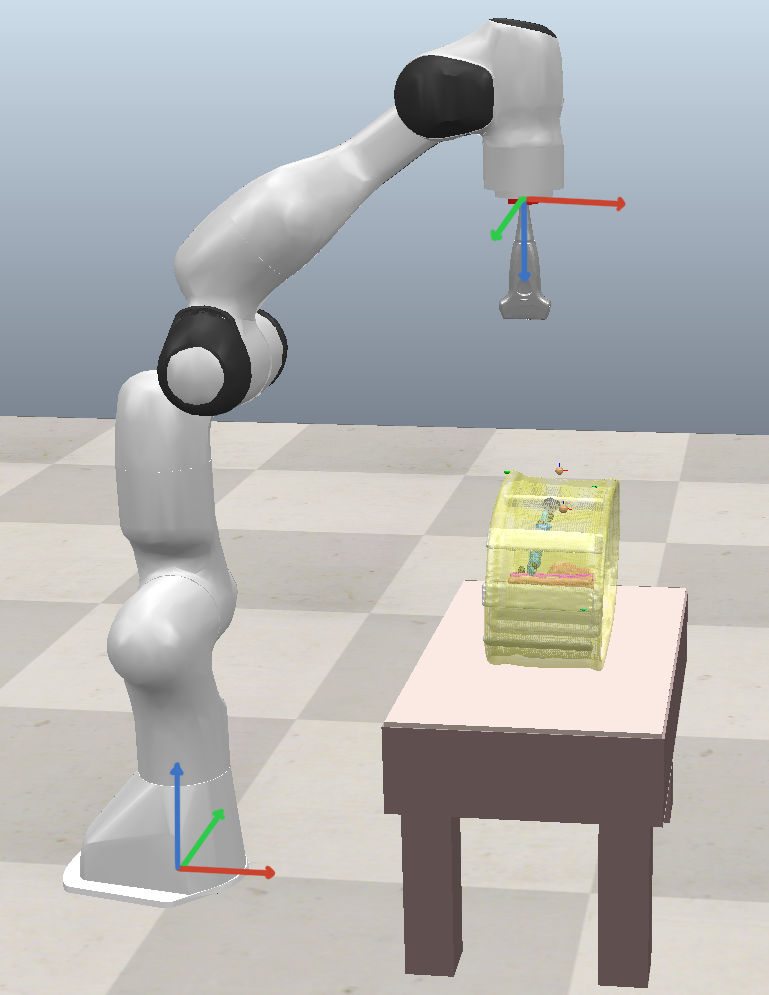
\includegraphics[width=0.8\textwidth]{Robot_with_RF.png}
    \captionof{figure}{World Frame and End-effector frame}
    \label{Robot_standing}
\end{minipage}
\vspace{1cm}
\newline
It is important to note that the final Euler angle ($\psi$) only describes the orientation around the probe's approach axis. In order to maintain a simpler Jacobian computation, the last rotation around the approach direction has not been used.
\\
The above mentioned representation has a singularity for $\theta = \pi$, that is when the z axis of the end-effector is vertical. To enable the use of this configuration during scans, a threshold has been implemented: when the configuration approaches $\theta = \pi$, the task over $\phi$ becomes ambiguous (is no longer possible to determine $\phi$ because of the representation singularity) and the gains of $\phi$ are set to zero to maintain a vertical approach direction for the end-effector and ignore the task for $\psi$. Several precautions have been taken in order to avoid sudden reconfigurations of the robot’s end-effector.
\\
To leverage the redundancy of the manipulator, a Task Augmentation technique was implemented, which involves extending the Analytic Jacobian to incorporate all tasks giving them equal priority.
By doing so, the manipulator can handle multiple objectives simultaneously without compromising task performance, whenever the tasks are compatible with each other. This approach not only optimizes control but also enhances safety, as it reduces the risk of abrupt movements. The ability to manage competing tasks efficiently helps maintain smooth, stable operations, especially in safety-critical environments like teleoperated procedures or tasks involving human interaction.
%%IMPEDENCE CONTROL DESIGN
\subsection{Impedence control design}
In tasks like teleoperated echography, it is essential to carefully control and minimize the interaction forces with the patient. To achieve this, an impedance control law was implemented with a specific configuration designed to further improve performance. The control law is designed to react to the error defined in Cartesian space ($e=r_{d}-r, \dot{e}=\dot{r}_{d}-\dot{r}$), by commanding the control input torque at the robot's joint level. It incorporates the dynamic model of the manipulator (excluding friction forces) to ensure the use of a reliable system model $\cite{Dynamic Identification}$. The control law assumes the interaction model with the environment follows the relationship:
$$
M(q)\ddot{q}+S(q,\dot{q})\dot{q}+g=u+J_{r}(q)^{T}F_{r}
$$
Where $F_{r}$ represents the generalized forces exerting work on $ \dot{r}$.
\\
The resulting control law is as follows:
$$
u=M(q)J_{r}(q)^{\#}\{\ddot{r}_{d}-\dot{J}_{r}(q)\dot{q}+ M_{m}^{-1}[D_{m}(\dot{r}_{d}-\dot{r})+K_{m}(r_{d}-r)]\}+S(q,\dot{q})\dot{q}+g+J_{r}(q)^{T}[M_{r}(q)M_{m}^{-1}-I]F_{r}
$$
To reduce the complexity of the model and simplify the controller, a further simplification has been adopted by setting the apparent inertia matrix $M_{m}$ equal to the natural Cartesian inertia of the robot, $M_{m}=M_{r}(q)$. The control law then simplifies to:
$$
u=M(q)J_{r}(q)^{\#}\{\ddot{r}_{d}-\dot{J}_{r}(q)\dot{q}\}+S(q,\dot{q})\dot{q}+g+J_{r}(q)^{T}[D_{m}(\dot{r}_{d}-\dot{r})+K_{m}(r_{d}-r)]
$$
Additionally, a damping term for joint velocities is introduced to reduce excessive self-motion in the joint space, which could otherwise compromise safety of the patient. The final control law becomes:
$$
u=M(q)J_{r}(q)^{\#}\{\ddot{r}_{d}-\dot{J}_{r}(q)\dot{q}\}+S(q,\dot{q})\dot{q}+g+J_{r}(q)^{T}[D_{m}(\dot{r}_{d}-\dot{r})+K_{m}(r_{d}-r)]-D_{q}\dot{q}
$$
Where $K_{m}, D_{m}$ and $D_{q}$ are the diagonal, positive definite gain matrices.
\\
Particular precautions have been taken with the $K_{z}$ component of the gain matrix $K_{m}$. To achieve more compliant behavior along the $z$ axis (aligned with the probe), the value of $K_{z}$ is set lower than those of  $K_{x}$ and $K_{y}$, where less significant contact is expected. These adjustments help ensure a safer and more comfortable scan, maintaining the compliant behavior of the manipulator when interacting with the patient at all times.
%%CONTROL MODALITIES
\subsection{Control modalities}
While predefined trajectories can be commanded, allowing the operator to make precise, fine adjustments to the end-effector’s pose can improve the quality of the scan and possibly yields better results. Specifically, the position and orientation of the robot’s end-effector can be modified in real time using external devices, such as an Xinput-compatible controller. This enables the operator to precisely adjust the echographic probe during the scan for more detailed analysis.
\\
Additionally, a GUI has been implemented to allow similar adjustments to the position and orientation using a mouse. Through the GUI, the operator can also adjust each component of the gain matrices $K_{m}, D_{m}$ and $D_{q}$ offering greater control over the system as shown in Figure $\ref{GUI}$.
\begin{figure}[h]
    \centering
    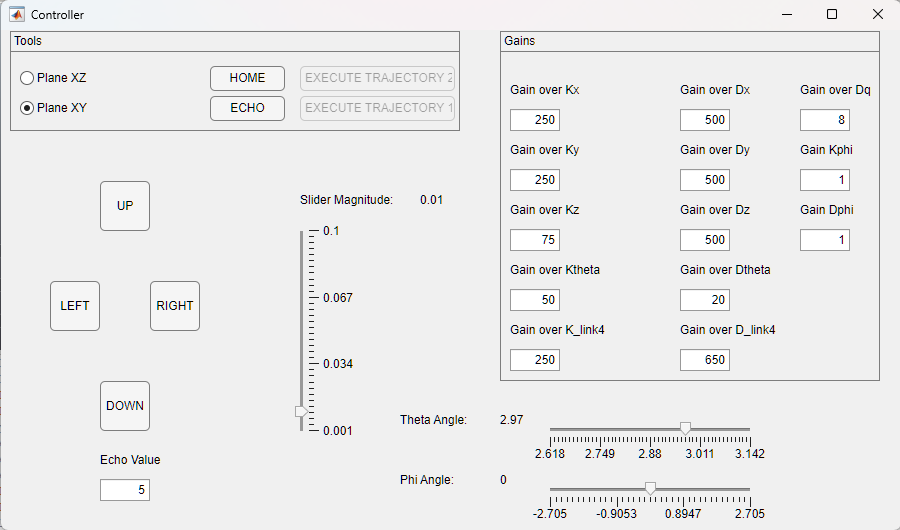
\includegraphics[width=0.7\textwidth]{New_gui.png}  
    \caption{GUI}
    \label{GUI}
\end{figure}
\newline
Although the operator can manually adjust the end-effector’s position, several safety precautions have been implemented to ensure patient protection. Specifically, a shared control protocol has been introduced by setting a safety threshold: if the force sensor detects a force along the Z-axis exceeding this threshold, the control system prevents any further increase in force in that direction. Additionally, to avoid commanding a reference position too deep into the patient—which would generate excessive force—a maximum allowable distance between the end-effector and the patient has been established.

\subsection{Trajectories}

\subsubsection{Regulation}
The main control approach works on a shared control architecture where the human operator controls a modifiable desired task vector (with a cartesian part, orientation and a restriction for the height of the fourth joint ), in the 3D-space and adopting a regulation law the robot converges to the specified task position. The transient quality and speed depends on the gains  for each task. Tuning the gains was a crucial step: accurate task tracking was needed with a sufficiently damped movement in order to avoid the possibility of harming the patient.
\\The implemented regulation control is the following:
$$u=M(q)J_{r}(q)^{\#}\{-\dot{J}_{r}(q)\dot{q}\}+S(q,\dot{q})\dot{q}+g+J_{r}(q)^{T}[-D_{m}\dot{r}+K_{m}(r_{d}-r)]-D_{q}\dot{q}$$
\\
Crucial precautions were taken on the update system of the desired task. Initially, a starting configuration is defined, from this point onward, control is handed over to the operator, who, using one of the previously mentioned control modalities, can update the desired task in real-time, except for the control of the height position of the fourth joint.
\newline
\begin{itemize}
\item{\textbf{Using the GUI:}} 
\\The integrated Matlab GUI allows the operator to control the Cartesian coordinates by incrementing the starting values. The magnitude of the increments can be adjusted via a slider. The increments are applied along the three axes of the world reference frame Additionally, the GUI provides two sliders to adjust the orientation by modifying both the $\theta$ and $\phi$ angles (as reported in Figure \ref{GUI}).
\item{\textbf{Using the Controller:}} 
\\Similar mechanics are used when utilizing a controller. The Cartesian reference position is updated proportionally to the displacement of the left analog stick in the X and Y directions. The Z position is controlled using  the two back triggers. $\theta$ is adjusted by two buttons that increment or decrement its value, while $\phi$ is controlled by the other analog stick, enabling circular movement based on the angle of inclination, providing a highly intuitive response.
\end{itemize}
\newpage
\subsubsection{Echo modality}
To ensure the echography is performed safely and accurately, it is essential to first establish contact with the patient using a constant, predetermined force. This process must be done gradually as the robot approaches the patient to avoid potential collisions, especially if the operator inadvertently commands a large movement toward the patient.\\
For a smooth and safe procedure, a method was implemented to gradually guide the probe into the operational workspace. The probe is moved slowly toward the patient while continuously monitoring the force sensor output. Once the sensor detects a specified threshold, the approach is complete, allowing the operator to proceed with the ultrasound, either manually or along a predefined trajectory.
\begin{figure}[H]
    \centering
    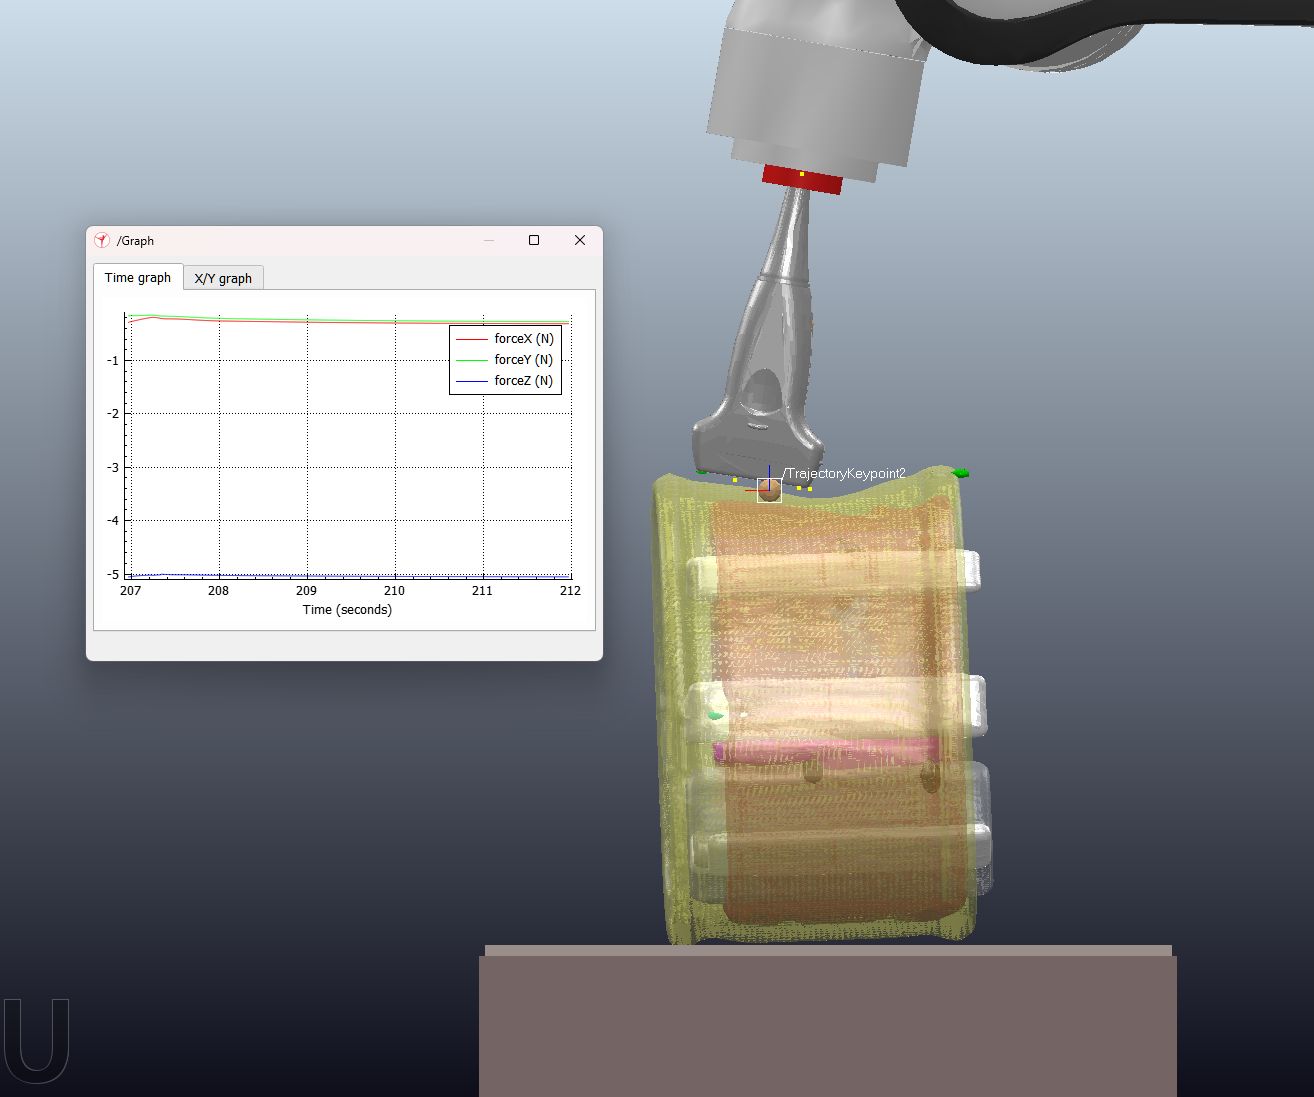
\includegraphics[width=0.7\textwidth]{Echo_mode.png}  
    \caption{Echo mode}
    \label{Echo}
\end{figure}
\hspace{-0.53cm}The plot of the torque efforts, the task errors and the Force measured when executing the trajectory are reported below:
\begin{figure}[H]
    \centering
    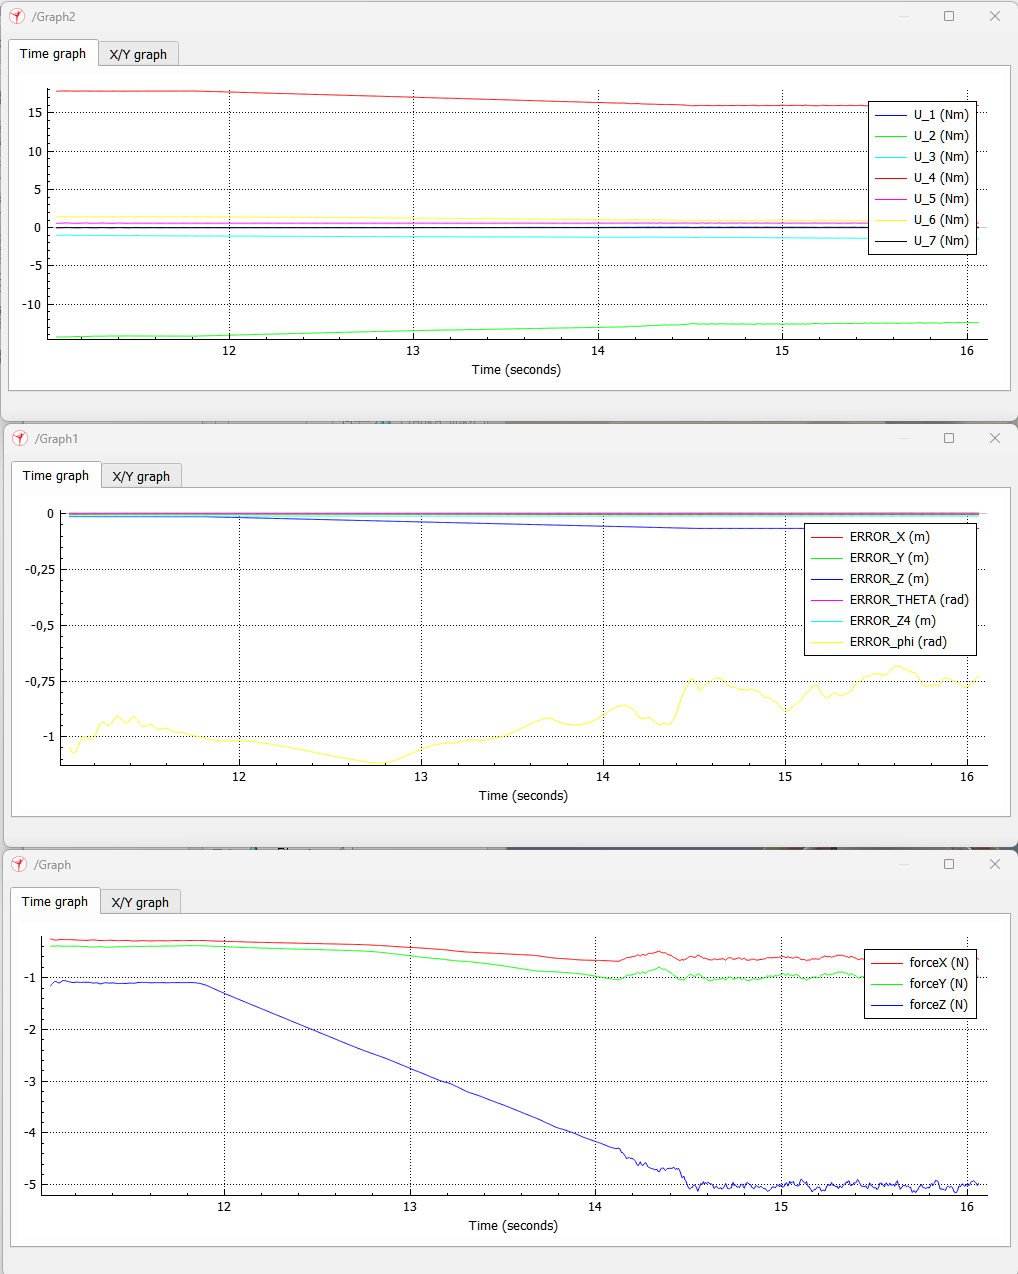
\includegraphics[width=0.7\textwidth]{echo_graphs.png}  
    \caption{Torque efforts, task errors and measured Forces plots for echo trajectory}
    \label{Echo}
\end{figure}

\subsubsection{Linear trajectory}
The first predefined executable trajectory is a linear cartesian path expressed between two adjustable points in the space.
The trajectory is expressed as a 6-component task, changing in time with a sinusoidal form along the y component of the reference task. while maintaining constant the initial configuration realized by the operator before executing this specific trajectory. The sinusoidal trajectory is bounded in amplitude by taking into account the two editable points’ Y coordinates.\\
The resulting trajectory will be defined as:
$$r_{d}=\begin{pmatrix}
r_{d1}\\
r_{d2}+A\cdot sin(\pi \frac{t}{T})\\
r_{d3}\\
r_{d4}\\
r_{d5}\\
r_{d6}\\
\end{pmatrix},
\quad \dot{r}_{d}=\begin{pmatrix}
0\\
A\frac{\pi}{T}\cdot cos(\pi \frac{t}{T})\\
0\\
0\\
0\\
0\\
\end{pmatrix},
\quad \ddot{r}_{d}=\begin{pmatrix}
0\\
-A(\frac{\pi}{T})^{2}\cdot sin(\pi \frac{t}{T})\\
0\\
0\\
0\\
0\\
\end{pmatrix}
$$
\newline
Where $T$ is the total execution time.
\\
Tracking is ensured using a slightly modified version of the previously mentioned regulation control law introducing a desired acceleration and velocity at each timestamp. Following a standard impedance design.
$$
u=M(q)J_{r}(q)^{\#}\{\ddot{r}_{d}-\dot{J}_{r}(q)\dot{q}\}+S(q,\dot{q})\dot{q}+g+J_{r}(q)^{T}[D_{m}(\dot{r}_{d}-\dot{r})+K_{m}(r_{d}-r)]-D_{q}\dot{q}
$$
Below, we present the plots of joint torque, task error, and force measurements, which are useful for evaluating the performance along the trajectory:
\begin{figure}[H]
    \centering
    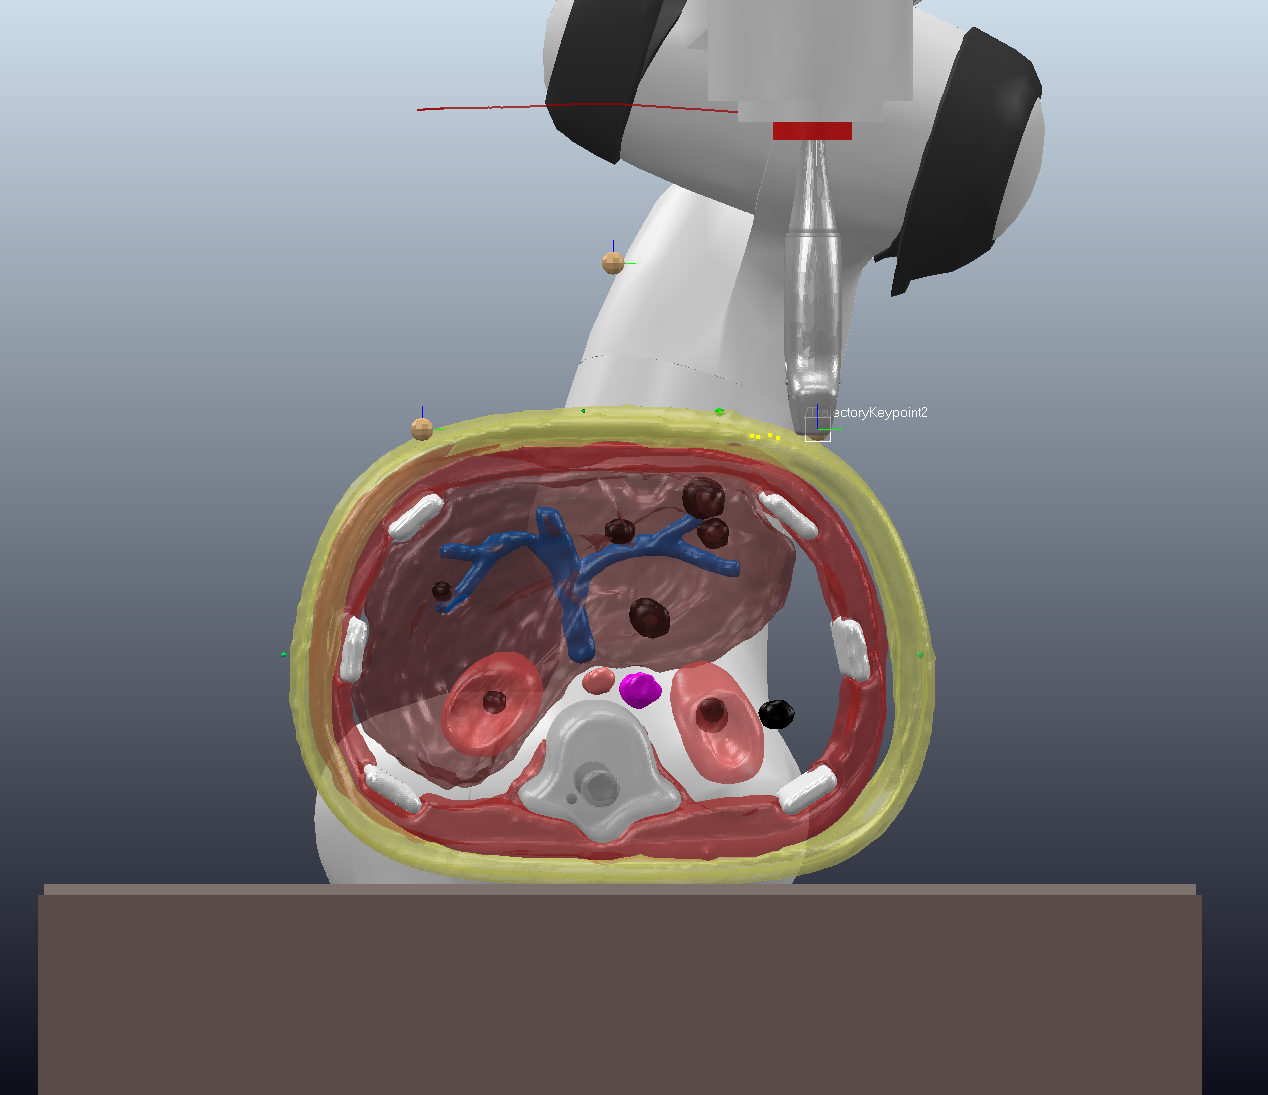
\includegraphics[width=0.5\textwidth]{Linear_Trajectory.png}  
    \caption{Linear trajectory}
    \label{lin}
\end{figure}
\begin{figure}[H]
    \centering
    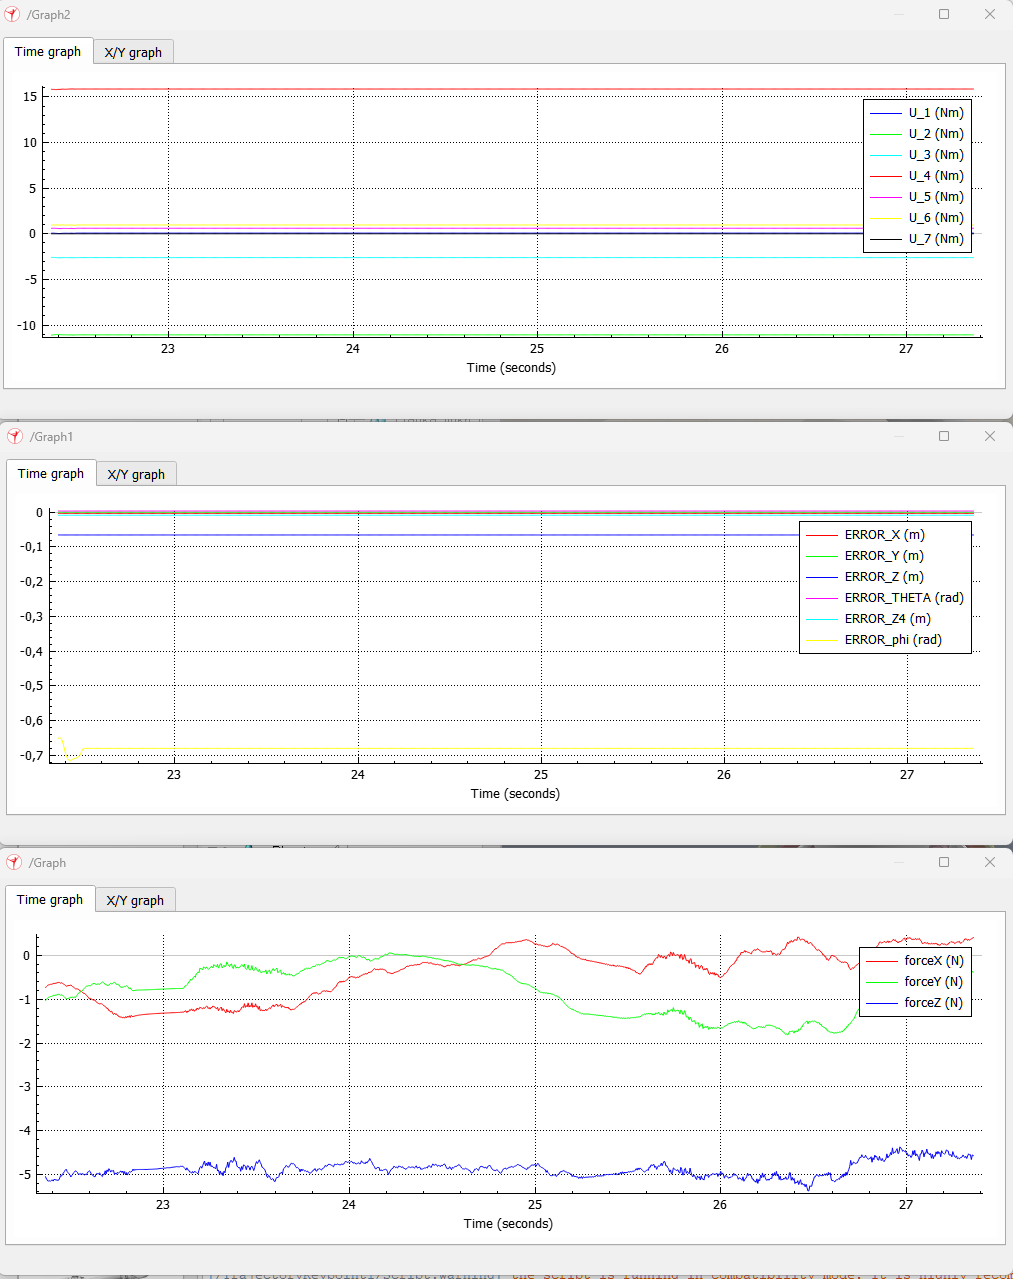
\includegraphics[width=0.7\textwidth]{Linear_graphs.png}  
    \caption{Torque efforts, task errors and measured Forces plots for linear trajectory}
    \label{graphs}
\end{figure}

\subsubsection{Wrist trajectory}
The second prefixed executable trajectory involves end-effector orientation, where the two task angles change over time. Due to the singularity that occurs in the ZYZ Euler angle representation when $\theta =\pi$ (corresponding to the probe's vertical downward configuration),the trajectory has been splitted into multiple steps in order to avoid fast reconfiguration near  the singularity.\\
The trajectory is split in two phases:, the first phase is  designed to move the $\theta$ angle far enough from the singularity, and the second part realizes the sinusoidal movement for the $\phi$ angle.
Lastly, the robot returns to the initial configuration.
\newline
Then the main trajectory for the $\phi$ angle considers a constant value of theta far enough from the singularity (2.97 rad) obtained in the previous steps.
$$r_{d}=\begin{pmatrix}
r_{d1}\\
r_{d2}\\
r_{d3}\\
r_{d4}\\
r_{d5}\\
C\cdot sin(2\pi \frac{t}{T})\\
\end{pmatrix},
\quad \dot{r}_{d}=\begin{pmatrix}
0\\
0\\
0\\
0\\
0\\
2C\frac{\pi}{T}\cdot cos(2\pi \frac{t}{T})\\
\end{pmatrix},
\quad \ddot{r}_{d}=\begin{pmatrix}
0\\
0\\
0\\
0\\
0\\
-C(2\frac{\pi}{T})^{2}\cdot sin(2\pi \frac{t}{T})\\
\end{pmatrix}
$$
\newline
Where $T$ is the total execution time.\\
Below, we present the plots of joint torque, task error, and force measurements, which are useful for evaluating the performance along the trajectory:\\
\begin{figure}[H]
    \centering
    \includegraphics[width=0.7\textwidth]{wrist_traj.png}  
    \caption{Wrist trajectory}
    \label{wrist_traj}
\end{figure}

\begin{figure}[H]
    \centering
    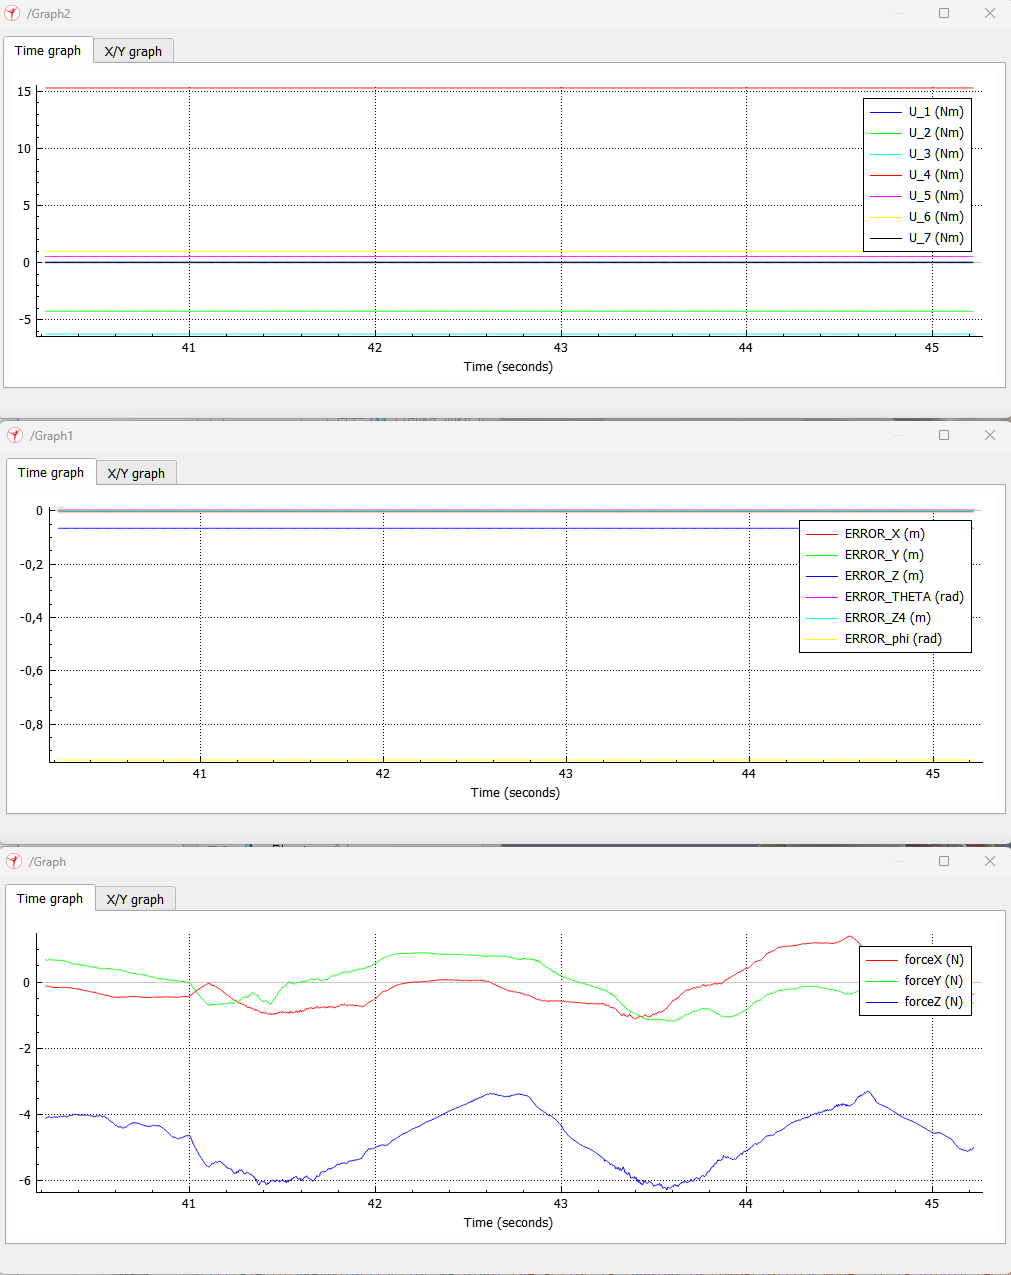
\includegraphics[width=0.67\textwidth]{wrist_graphs.png}  
    \caption{Torque efforts, task errors and measured Forces plots for wrist trajectory}
    \label{wrist_graphs}
\end{figure}

\section{Conclusion}
In conclusion, a comprehensive framework integrating various tools and a shared control approach has been developed in this project. One of the primary objectives was to leverage the robot’s advantages, such as precision and accuracy, which ultimately contribute to efficiency and patient safety, while still allowing the operator to take control and guide the scanning operation when needed. The shared control method ensures a balance between automated precision and human intervention, allowing the operator to manually adjust the robot’s actions without compromising safety. To achieve this, both the robot’s redundancy and torque-level control were utilized, enabling smooth transitions between automated tasks and operator-commanded adjustments. Finally, the preferred control strategy is the impedance control law, which facilitates smooth and safe interaction between the robot and the patient, adapting to external forces and ensuring compliant and responsive behavior during the scanning process.



\section{Future works}
The project has exciting opportunities for growth and several potential improvements remain to be implemented.
\begin{itemize}
\item One such enhancement is the integration of force feedback into the controller. By utilizing the motors that produce vibration within the controller, it could be possible to generate vibrations proportional to the force sensed along the Z-axis or to the magnitude of the force vector measured by the force sensor. This would provide the operator with tactile feedback, offering a better understanding of the interaction between the robot’s end-effector and the patient, thereby enhancing control and safety during operations.
\item A master-slave control system could be implemented to offer an alternative input method. This approach would allow the operator to more directly mimic the end-effector’s position, providing a simpler and more intuitive way to control the robot, thereby improving the precision and ease of operation. One potential system for this is the Geomagic, which not only offers intuitive control but also provides force feedback, giving the operator a tactile sense of the interaction between the robot and its environment.
\item To minimize errors during task execution, alternative approaches to task augmentation could be explored. One such method is task prioritization, which allows for the assignment of priority levels to different tasks. This would enable the system to minimize errors in critical tasks while accepting slightly larger errors in less crucial ones.
\end{itemize}


\addcontentsline{toc}{section}{References}
\begin{thebibliography}{9}

\bibitem{Dynamic Identification}
  C. Gaz , M. Cognetti , A.Oliva ,
P. Robuffo Giordano , and A. De Luca,
  \emph{“Dynamic Identification of the Franka Emika Panda
Robot With Retrieval of Feasible Parameters
Using Penalty-Based Optimization”},
   IEEE ROBOTICS AND AUTOMATION LETTERS, VOL. 4, NO. 4, OCTOBER 2019.
   
\bibitem{articolo prof}
 M. Dyck , A. Weld , J. Klodmann , A. Kirst, L. Dixon, G. Anichini ,
S. Camp, A. Albu-Schäffer, and S. Giannarou,
  \emph{“Toward Safe and Collaborative Robotic Ultrasound
Tissue Scanning in Neurosurgery”},
  IEEE TRANSACTIONS ON MEDICAL ROBOTICS AND BIONICS, VOL. 6, NO. 1, FEBRUARY 2024.
  
\bibitem{Colleagues}
  M. Germano, D. Gasperini, F. Cocci, C. Borzillo,
  \emph{IMPLEMENTATION OF IMPEDANCE
CONTROL FOR A TELE-ECHOGRAPHIC SYSTEM},
Medical Robotics Final Project 2021/2022

\bibitem{TER}
A. Vilchis Gonzales, P. Cinquin, J. Troccaz1, A. Guerraz, B. Hennion, F. Pellissier, P. Thorel, F.
Courreges, A. Gourdon, G. Poisson, P. Vieyres, P. Caron, O. Mérigeaux, L. Urbain, C. Daimo,
S. Lavallée, P. Arbeille, M. Althuser, J. Ayoubi, B. Tondu, S. Ippolito,
  \emph{“TER: a system for robotic tele-echography”},
  W. Niessen and M. Viergever (Eds.): MICCAI 2001, LNCS 2208, pp. 326-334, 2001.
  
\bibitem{MELODY}
 \emph{“MELODY – Telerobotic ultrasound solution”},
 https://www.adechotech.com/products/
  
  \bibitem{OTELO}
F. Courreges, P. Vieyres and R. S. H. Istepanian,
  \emph{“Advances in robotic tele-echography services - the OTELO system”},
The 26th Annual International Conference of the IEEE Engineering in Medicine and Biology Society, 2004.
\end{thebibliography}
\vspace{2cm}
We extend our sincere gratitude to Professor Marilena Vendittelli and collaborator Marco Ferro that helped the team to solve issues and develop the final project.

\end{document}